\documentclass[12pt,a4paper]{article}
\usepackage[latin1]{inputenc}
\usepackage{float}
\usepackage{amsmath}
\usepackage{amsfonts}
\usepackage{amssymb}
\usepackage{graphicx}
\author{Luca Conterio - 920261\\
	Ibrahim El Shemy - 920174}
\date{A.Y. 2018/2019 - Prof. Di Nitto Elisabetta}



\title{%
	\textbf{\Huge{TrackMe}} \\
	\large \texttt{Design Document}
}

\begin{document}
	\begin{figure}
		\centering
		
\includegraphics[width=1.0\linewidth]{images/polimi}
	\end{figure}
	\maketitle

	\newpage
	\tableofcontents
	\newpage

	\section{Introduction}
	\subsection{Purpose}
	This document represents the \texttt{Design Document} (DD) for TrackMe software and contains a functional description of the system. We provide an overall guidance to the architecture of the system and it is therefore addressed to the software development team.
	\subsection{Scope}
	\texttt{TrackMe} is a company that wants to develop a software-based service allowing third parties to monitor the location and health status of individuals. Hence, the system has to be composed by two specific services:
	\begin{itemize}
	 	\item \textbf{Data4Help}\\\\
	 	This service supports the registration of individuals who agree that TrackMe acquires their data (through electronic devices such as smartwatches).
	 	\item \textbf{AutomatedSOS}\\\\ 
	 	This service is oriented to elderly people: monitoring their health status parameters, the system can send to the location of the customer an ambulance when some parameters are below certain thresholds, guaranteeing a reaction time of less than 5 seconds from the time the parameters get lower than the threshold.
	\end{itemize}
 	\subsection{Definitions, Acronyms and Abbreviations}
 		\subsubsection{Definitions}
 		\subsubsection{Acronyms}
 			\begin{itemize}
 				\item \textbf{DD}: Design Document
 				\item \textbf{RASD}: Requirments Analysis and Specification
 				\item \textbf{ERP}: Enterprise Resource Planning
 				\item \textbf{DMZ}: Demilitarized Zone
 				\item \textbf{RAPS}: Reliable Array of Partitioned Service
 			\end{itemize}
 		\subsubsection{Abbreviations}
	\subsection{Document Structure}
		\begin{itemize}
			\item \textbf{1 Introduction}\\\\
			This section introduces the Design Document. It explains the Purpose, the Scope and the framework of the document.
			\item \textbf{2 Architectural Design}\\\\
			This section is focused on the main components used for this system and the relationship between them, providing information about their deployment and how they operate. It also focuses on the architectural styles and the design patterns adopted for designing the system.
			\item \textbf{3 User Interface Design}\\\\
			This section provides an overview on how the User Interface will look like and furthermore gives a more detailed extension using UX and BCE diagrams.
			\item \textbf{4 Requirments Traceability}\\\\
			This section explains how the requirements defined in the RASD map to the design elements defined in this document.
			\item \textbf{5 Implementation, Integration and Test Plan}
		\end{itemize}
\newpage
\section{Architectural Design}
	\subsection{High Level Components and their Interactions}
	\begin{figure}[h]
		\centering
		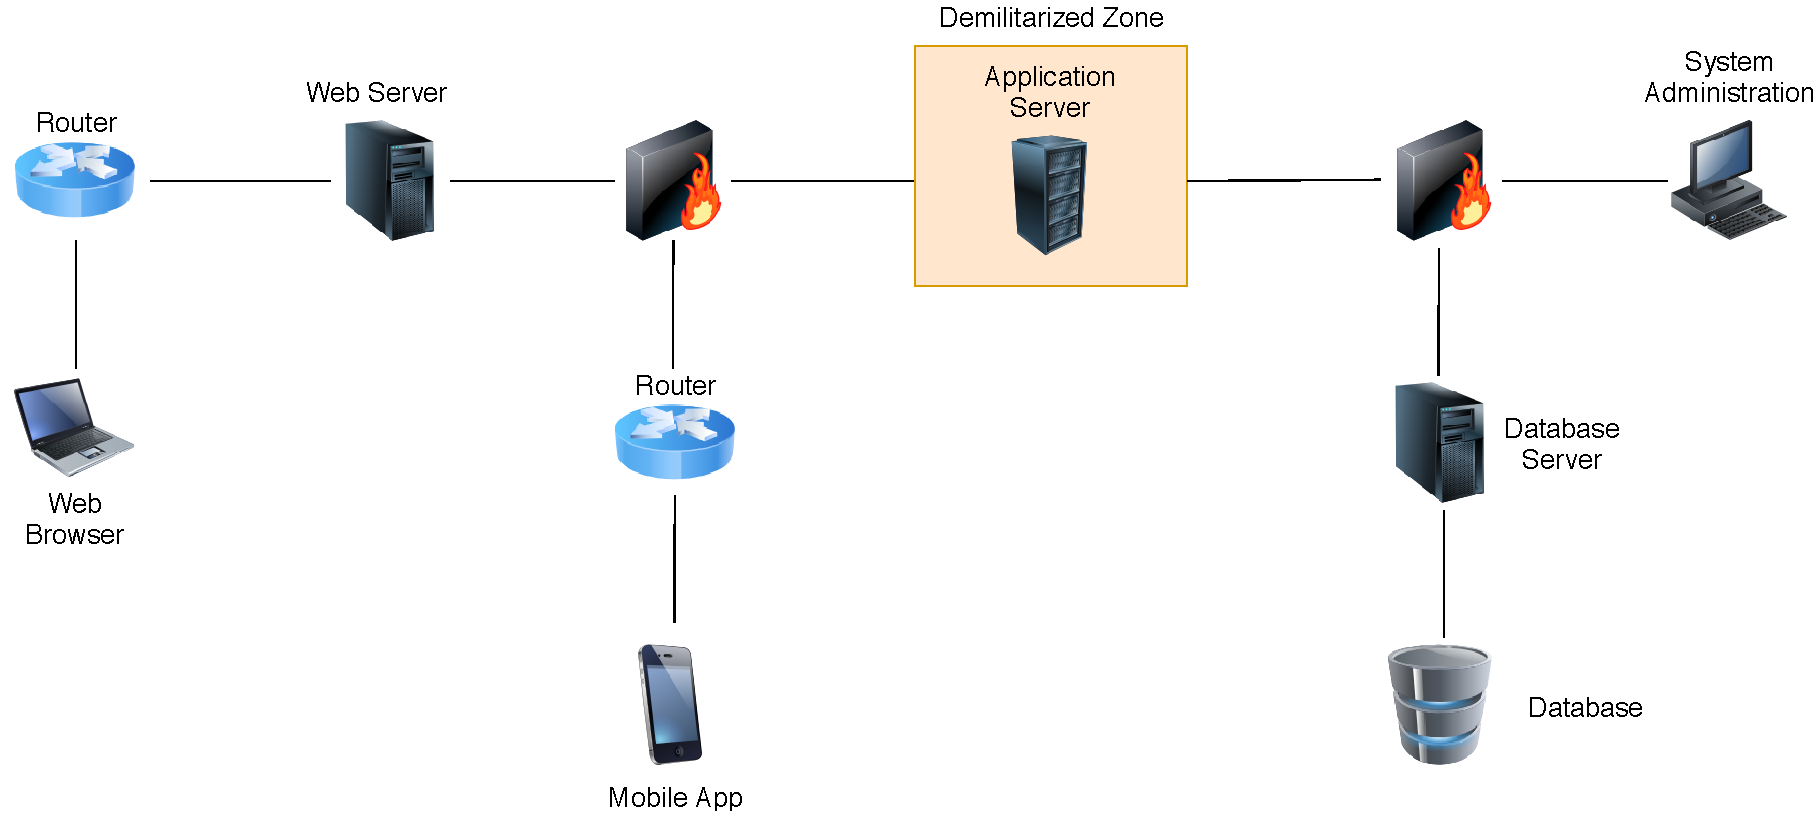
\includegraphics[height=0.5\linewidth]{images/high_level_diag}
		\caption{High Level System Structure}
		\label{fig:highleveldiag} 
	\end{figure}


The architecture of our system can be streamlined into 3 logic layers:
	\begin{itemize}
		\item \textbf{Presentation Layer}\\ 
		This layer can be divided into the Client tier (that includes the Web App and the Mobile App) and the Web tier. Third parties can access the system's functionalities and Users' information to which they are subscribed to through the Web Server. 
		\item \textbf{Application Layer}\\
		Users logged into the Mobile Application can access the system's functionalities and communicate with the Application Server, located in a Demilitarized Zone (DMZ), directly.
		\item \textbf{Data Layer}\\
		On top of that, we have the Database Server and the Database itself, where data about registered Users and Third Parties are stored and managed.
	\end{itemize}
	System Administration is implemented through a third-party ERP solution, hence we do not provide information about its implementation.
	
\section{Component View}
	\subsection{High Level Component Diagram}	
	\subsection{Deployment View}
	For the deployment of the system, we opted for a 4-tier architecture composed as follows:
	\begin{itemize}
		\item \textbf{Tier 1}\\
		This tier is composed by the Client (implemented as a Thin Client), that includes the Web App (run by a web browser) and the Mobile Application (run by smartphones). 
		\item \textbf{Tier 2}\\
		This tier is composed by the Web Server, whose main functionality is to store, process static content and deliver web pages to the Clients. For this reason, we opted for NGINX, that guarantees better perfomances for static content processing. It can be also configured as a load balancer, in order to better handle multiple connections.
		\item \textbf{Tier 3}\\
		This tier corresponds to the Application Server, that provides both facilities to create web applications and a server environment to run them. We opted for WildFly (v. 12.0.0 or recent versions - previously JBoss) since it fully implements all Java EE specifications.
		\item \textbf{Tier 4}\\
		This tier corresponds to the Database Server on which the DBMS is running. We opted for MySQL (v. 8.0.12) since it is one of the most secure and reliable database management system used in popular web applications and guarantees scalability and high performance.
	\end{itemize}

	As mentioned briefly in the RASD (sections 3.9.2, 3.9.5), our system has to rely on a RAPS architecture, in order to prevent unavailability of some functionalities in case of breakdowns. This architecture consists in a partitioned and redundant structure: servers are cloned to achieve this objective.
	More precisly, multiple services are divided on different machines and each machine can access in turn to a copy of the stored data. Such architecture guarantees better availability and scalability and provides a high rate of maintainability: in case of breakdowns, it is sufficient to work on the damaged machine, without interfering with the other machines' tasks, while the specific service can still be perfomed. 
	In addition, if the system is willing to expand some services, it is sufficient invest on the specific partition associated to that service.
	
		\begin{figure}[H]
			\centering
			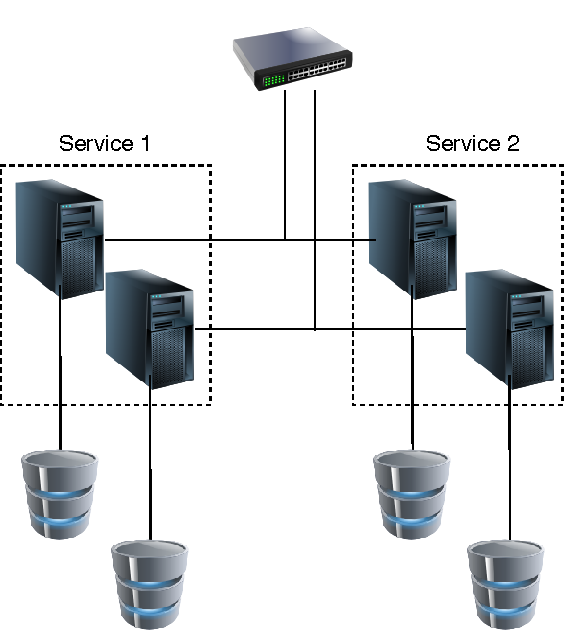
\includegraphics[width=0.6\linewidth]{images/raps}
			\caption{RAPS Architecture}
			\label{fig:raps}
		\end{figure}
		

		\begin{figure}[H]
		\centering
		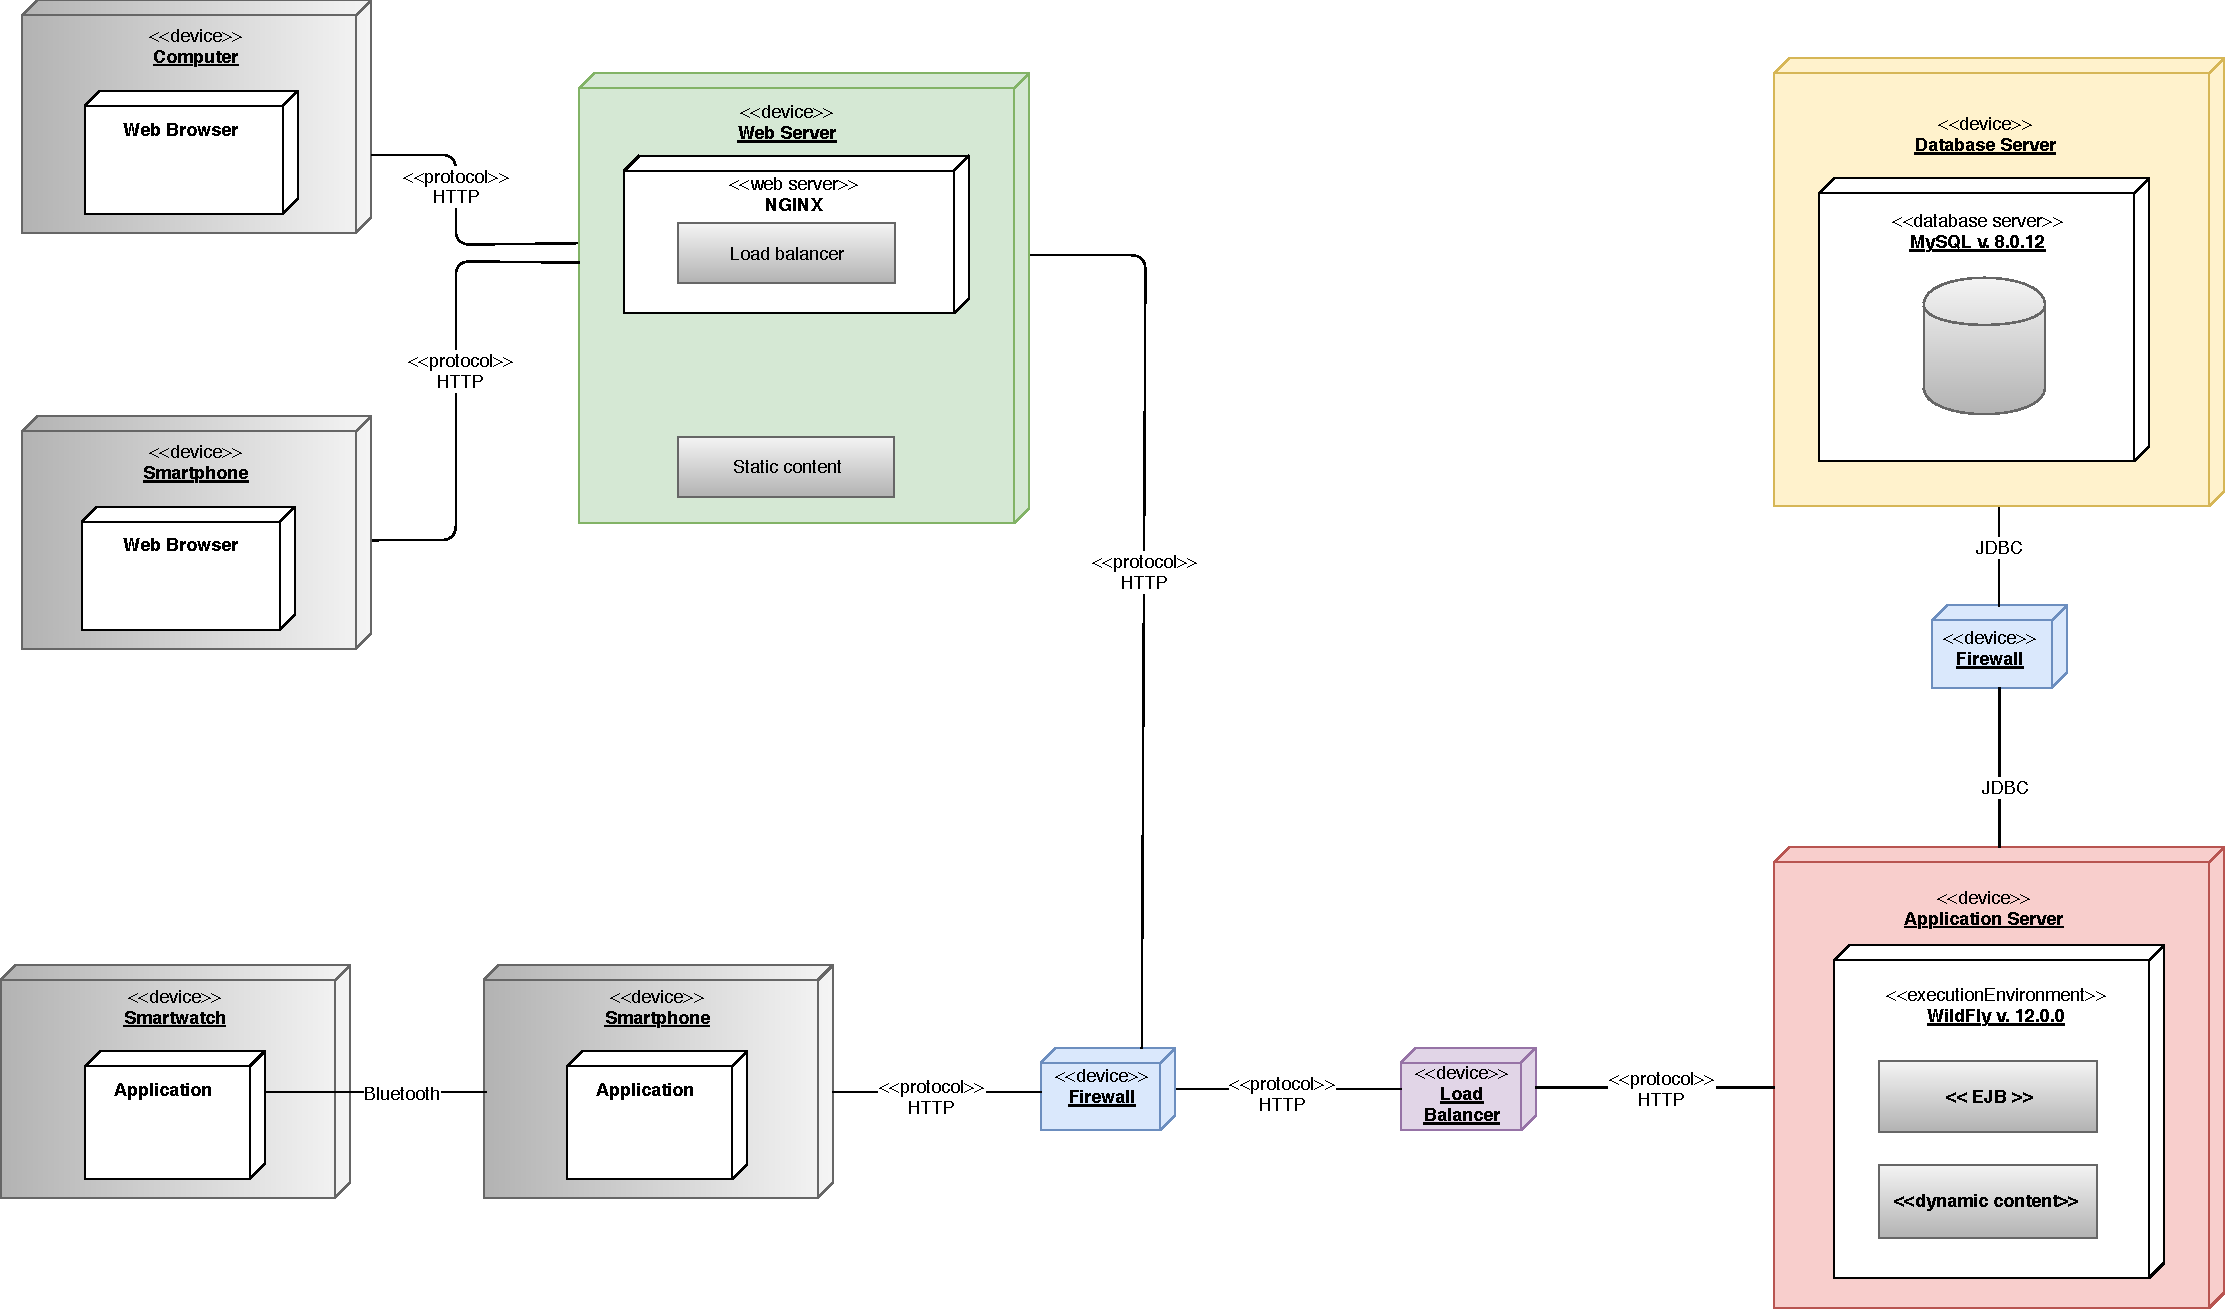
\includegraphics[width=1.0\linewidth]{images/deployment_diagram}
		\caption{Deployment View Diagram}
		\label{fig:deploymentdiagram}
		\end{figure}
	\subsection{Runtime View}
		



	\newpage
	%\section{Appendix}
	\section{Effort Spent}
	\begin{itemize}
		\item Luca Conterio
		\begin{center}
			\begin{tabular}{| c | c | c |}
				\hline
				Day & Subject & Hours \\ \hline
				19/11 & High Level Components & 1.30 \\ \hline
				22/11 & Deployment View & 2.30 \\ \hline
			\end{tabular}
		\end{center}

		\item Ibrahim El Shemy
		\begin{center}
			\begin{tabular}{| c | c | c |}
				\hline
				Day & Subject & Hours \\ \hline
				19/11 & Introduction of the document & 1.30 \\ \hline
				22/11 & Deployment View & 2.30 \\ \hline
			\end{tabular}
		\end{center}
	\end{itemize}
	\section{References and Used Tools}
		\subsection{Reference Documents}
			\begin{itemize}
				\item Specification Document "Mandatory Project Assignment A.Y. 2018/2019"
			\end{itemize}
		\subsection{Tools}
			\begin{itemize}
				\item \textbf{Draw.io}: \texttt{https://www.draw.io/}
				\item \textbf{TeXStudio}: \texttt{http://www.textstudio.org/}
				\item \textbf{Github}: \texttt{https://github.com/}
			\end{itemize}
		
\end{document}
